\documentclass[letterpaper,11pt]{article}
\usepackage[utf8x]{inputenc}
\usepackage{enumerate}
\usepackage{enumitem}
\usepackage{fullpage}
\usepackage{amsmath}

\usepackage{pgf}
\usepackage{tikz}
\usetikzlibrary{arrows,shapes,trees}

%opening
\title{Midterm Exam \\ Classical Mechanics \\ Physics 601 (Fall 2013)}
\date{Due by 9:30am on Thursday October 17, 2013}

\begin{document}

\maketitle

\paragraph*{Lagrangian Mechanics}
\begin{enumerate}
 \item Two masses $m_1$ and $m_2$ are connected by a string with fixed length passing through a hole in a smooth table, so that $m_1$ rests on the table and $m_2$ hangs suspended and moves only in the vertical direction.  Consider the motion until $m_1$ reaches the hole.
 \begin{itemize}
  \item Write down the Lagrangian and the equations of motion for this system. Interpret the first integral you encounter.
  \item Under what condition will the hanging mass remain stationary?
  \item Starting from this stationary situation, the mass $m_2$ is pulled down slightly and released again. Investigate the resulting small oscillations in the vertical position of $m_2$.
  \item Calculate the tension in the string for stationary motion using the method of the Lagrange multipliers.
 \end{itemize}
\end{enumerate}

The mass $m_1$ on the table has polar coordinates $r$ and $\theta$; the mass $m_2$ is hanging from the hole with a length $z = l - r$.  We start from the Lagrangian $L = T - V$,
\begin{equation*}
 L = \frac{1}{2} m_1 (\dot{r}^2 + r^2 \dot{\theta}^2) + \frac{1}{2} m_2 \dot{r}^2 - m_2 g (l - r).
\end{equation*}
The equations of motion for $r$ and $\theta$ are then
\begin{eqnarray*}
 \frac{d}{dt} \left( \frac{\partial L}{\partial \dot{r}} \right) = (m_1 + m_2) \ddot{r} & = & \frac{\partial L}{\partial r} = m_1 r \dot{\theta}^2 + m_2 g, \\
 \frac{d}{dt} \left( \frac{\partial L}{\partial \dot{\theta}} \right) = \frac{d}{dt} \left( m_1 r^2 \dot{\theta} \right) & =  & \frac{\partial L}{\partial \theta} = 0.
\end{eqnarray*}
The second equation implies constant angular momentum $\ell = m_1 r^2 \dot{\theta}$.  After eliminating $\dot{\theta}$ from the first equation, we find
\begin{equation*}
 (m_1 + m_2) \ddot{r} - \frac{\ell^2}{m_1 r^3} + m_2 g = 0.
\end{equation*}

When the mass is stationary, the time-derivatives of $r$ will be zero in this equation, or
\begin{equation*}
 \frac{\ell^2}{m_1 r^3} = m_2 g,
\end{equation*}
With $\dot{\theta} = \omega_0$ this results in an equilibrium radius $r_0 = \frac{m_2 g}{m_1 \omega_0^2}$.  Deviations from this equilibrium, $r = r_0 + \Delta r$, result in a differential equation
\begin{equation*}
 (m_1 + m_2) \Delta\ddot{r} - \frac{\ell^2}{m_1} (r_0 + \Delta r)^{-3} + m_2 g = 0.
\end{equation*}
Expanding to first order in $\Delta r$ results in
\begin{equation*}
 (m_1 + m_2) \Delta\ddot{r} - \frac{\ell^2}{m_1} r_0^{-3} (1 - 3 \frac{\Delta r}{r_0}) + m_2 g = 0,
\end{equation*}
where the constant terms drop out by definition of $r_0$, and we are left with a harmonic oscillator equation with frequency
\begin{equation*}
 \omega = \sqrt{\frac{3 m_1}{m_1 + m_2}} \omega_0.
\end{equation*}

If we keep the third coordinate $z$ independent and impose the constraint $z = l - r$, or $\dot{z} = -\dot{r}$, with Lagrange multiplier $\lambda$, then we find the equations
\begin{eqnarray*}
 (m_1 + m_2) \ddot{r} - m_1 r \dot{\theta}^2 + \lambda & = & 0, \\
 m_1 r^2 \dot{\theta} & = & \ell, \\
 m_2 \ddot{z} + m_2 g + \lambda & = & 0.
\end{eqnarray*}
For the stationary condition, $\dot{r} = 0$, this results in $\lambda = m_1 r_0 \omega_0^2 = m_2 g$, \textit{i.e.} the tension in the string is equal to the weight of the second mass, as expected.


\begin{enumerate}[resume]
 \item A particle of mass $m$ in a uniform gravitational field is constrained to move on a helical wire with height $z = a\theta$ and radius $r = b$ in cylindrical coordinates.
 \begin{itemize}
  \item Write down the Lagrangian and the equations of motion for this system.
  \item Solve the equations of motion if at $t = 0$ the mass is at $z = 0$.
  \item Find the forces of constraint using the method of the Lagrange multipliers.
 \end{itemize}
\end{enumerate}

The Lagrangian for this system as a function of $\theta$, $z$ and $r$ is
\begin{equation*}
 L = \frac{1}{2} m \left( \dot{r}^2 + r^2 \dot{\theta}^2 + \dot{z}^2 \right) - m g z,
\end{equation*}
with constraints $z = a \theta$ and $r = b$, or correspondingly $\dot{z} = a\dot{\theta}$ and $\dot{r} = 0$.  The equations of motion are then
\begin{eqnarray*}
 m \ddot{r} - m r \dot{\theta}^2 + \lambda_2 & = & 0, \\
 m r^2 \ddot{\theta} + 2 m r \dot{r} \dot{\theta} - a \lambda_1 & = & 0, \\
 m \ddot{z} + m g + \lambda_1 & = & 0.
\end{eqnarray*}

When taking into account the constraints, we can eliminate $r$ and $z$ to find a single equation of motion for $\theta$,
\begin{equation*}
 m (a^2 + b^2) \ddot{\theta} + m g a = 0.
\end{equation*}
Solving this with the given initial conditions results in
\begin{equation*}
 \theta = - \frac{1}{2} g \frac{a}{a^2 + b^2} t^2.
\end{equation*}

When solving for $\lambda_1$ and $\lambda_2$ and plugging in the solution for $\theta$ we find
\begin{eqnarray*}
 \lambda_1 & = & - m g - m a \ddot{\theta} = - m g \frac{b^2}{a^2 + b^2}, \\
 \lambda_2 & = & m \dot{\theta}^2 = - m g^2 \frac{a^2}{(a^2+b^2)^2} t^2.
\end{eqnarray*}
The interpretation of these forces is that $\lambda_1$ is the fraction of the gravitational force (or force of reaction from the wire on the bead) that is perpendicular to the helix.  The centripetal force is given by $\lambda_2$.


\begin{enumerate}[resume]
 \item A particle of mass $m$ suspended by a massless string of length $\ell$ is stationary in a gravitational field $g$.  It is struck by an impulsive horizontal blow, giving it an initial angular velocity $\omega$.  Introduce a Lagrange multiplier and prove the following statements:
 \begin{itemize}
  \item If $\ell\omega^2 < 2g$, the tension $\tau$ does not vanish and the particle does not reach the horizontal.
  \item If $2g < \ell\omega^2 < 5g$, the particle passes the horizontal and the string becomes slack before the particle comes to rest.
  \item If $5g < \ell\omega^2$, the string always remains taut and the particle executes periodic circular motion.
 \end{itemize}
 Discuss the role of the tension $\tau$ in the string by showing how these results are changed if the string is replaced by a rigid massless rod.
\end{enumerate}

We start with the Lagrangian for the simple pendulum in the coordinates $r$ and $\theta$ with constraint $r = \ell$,
\begin{equation*}
 L = \frac{1}{2} m (\dot{r}^2 + r^2 \dot\theta^2) + m g r \cos\theta.
\end{equation*}

With the Lagrange multiplier $\lambda$ the Euler-Lagrange equations are
\begin{eqnarray*}
 m \ddot{r} - mr\dot{\theta}^2 - mg\cos\theta & = & \lambda \\
 m r^2 \ddot{\theta} + 2mr\dot{r}\dot{\theta} + mgr\sin\theta & = & 0 \\
 r & = & \ell.
\end{eqnarray*}
The tension $\tau$ is given by the Lagrange multiplier $\lambda$ as
\begin{equation*}
 \tau = \lambda = m \ell\dot{\theta^2} + mg\cos\theta.
\end{equation*}
For small $\theta$ this is positive.

Since the Lagrangian does not depend on the time, the Hamiltonian $H = \frac{1}{2} m (\dot{r}^2 + r^2 \dot\theta^2) - m g r \cos\theta$ will be conserved.  At the lowest point, immediately after impact, the Hamiltonian is $H = \frac{1}{2} m \ell^2 \omega^2 - m g \ell$.

We can see that the tension $\tau$ will always be positive for $\theta < \frac{\pi}{2}$ and the string will remain taut for for angles below $\frac{\pi}{2}$.  If the pendulum swings with amplitude $\theta = \frac{\pi}{2}$ the Hamiltonian at the largest angle will be $H = 0$.  When $\ell \omega^2 < 2 g$ the pendulum will not swing higher than $\theta = \frac{\pi}{2}$.

Naively, if the pendulum swings with amplitude $\theta = \pi$ the Hamiltonian at the largest angle will be $H = m g \ell$, which would lead one to think incorrectly that the minimum value for $\ell\omega^2$ is now $4 g$.  However, while correct for a rigid massless rod, the tension $\tau$ is negative at $\theta = \pi$ when $\dot{\theta} = 0$ and the string is slack before it reaches this point.

To ensure that the tension is positive for $\theta = \pi$, we require that $\tau = m \ell\dot{\theta^2} - mg > 0$, or $\dot{\theta}^2 > \frac{g}{\ell}$.  This means that $H = \frac{1}{2} m \ell^2 \omega^2 - m g \ell > \frac{1}{2} m \ell^2\frac{g}{\ell} + m g \ell$ if $\ell\omega^2 > 5 g$.

Since a rigid massless rod can support the mass under both positive and negative tension, the initial angular velocity does not need to be as large.


\paragraph*{Hamiltonian Mechanics}
\begin{enumerate}[resume]
 \item Show that the transformation
 \begin{eqnarray*}
  Q & = & p + i \alpha q, \\
  P & = & \frac{1}{2i\alpha}(p-i\alpha q),
 \end{eqnarray*}
 is canonical and find a generating function.  Use this transformation to solve the simple linear harmonic oscillator problem.
\end{enumerate}

The Poisson brackets for the transformed coordinates $P$ and $Q$ are
\begin{eqnarray*}
 [P,P] & = & -\frac{1}{4\alpha^2} [p-i\alpha q,p-i\alpha q] = -\frac{1}{2\alpha^2} \left( [p,-\alpha q] + [-i\alpha q,p] \right) = 0, \\ \null
 [Q,Q] & = & [p+i\alpha q,p+i\alpha q] = [p,i\alpha q] + [i\alpha q,p] = 0, \\ \null
 [P,Q] & = & \frac{1}{2i\alpha} [p-i\alpha q,p+i\alpha q] = \frac{1}{2i\alpha} \left( [p,i\alpha q] - [i\alpha q,p] \right) = [p,q] = -1.
\end{eqnarray*}
Since the Poisson brackets are identical, the transformation must be canonical.

If we invert the transformation such that $p$ and $P$ are written as functions of $q$ and $Q$,
\begin{eqnarray*}
 p & = & Q-i\alpha q, \\
 P & = & \frac{1}{2i\alpha} (Q-2i\alpha q),
\end{eqnarray*}
and we require that $p = \frac{\partial F}{\partial q}$, we find $F(q,Q,t) = qQ - \frac{1}{2} i\alpha q^2 + f(Q)$ for any function $f(Q)$.  For this generating function we find $P = -\frac{\partial F}{\partial Q} = -q - f'{Q}$.  With the expression for $P$ above we must have $f(Q) = -\frac{1}{4i\alpha} Q^2$.  In summary,
\begin{equation*}
 F(q,Q,t) = qQ - \frac{1}{2} i\alpha q^2 - \frac{1}{4i\alpha} Q^2.
\end{equation*}

The transformed Hamiltonian of $H = \frac{1}{2} \left( p^2 + \alpha^2 q^2 \right)$ is $K = i\alpha PQ$.  This results in Hamilton's equations
\begin{eqnarray*}
 \dot{Q} & = & i\alpha Q, \\
 \dot{P} & = & -i\alpha P,
\end{eqnarray*}
with solution $Q = Q_0 \exp (i\alpha t)$ and $P = P_0 \exp (-i\alpha t)$.


\begin{enumerate}[resume]
 \item A particle moving in one dimension sees a force $F(t) = \lambda t$ that is linearly increasing with time.  Solve the equations of motion using Hamilton's principal function for the initial conditions $x(0) = 0$ and $p(0) = mv_0$.
\end{enumerate}

For the given force $F(t) = -\frac{dV}{dx}$ we require a potential $V(x) = -\lambda tx$.  The Hamiltonian becomes then $H = \frac{p^2}{2m} - \lambda tx$ and the Hamilton-Jacobi equation is
\begin{equation*}
 \frac{1}{2m}\left(\frac{\partial S}{\partial x}\right)^2 - \lambda tx + \frac{\partial S}{\partial t} = 0.
\end{equation*}
The separation is not possible in this form.  In order to separate the variables, we try to write the equation only in terms of $t$, not $x$, by adding a term $\frac{1}{2} \lambda xt^2$ to cancel the $\lambda tx$, and we also keep the rest of the generating function linear in $x$ so no $x$ dependence remains after a single differentiation:
\begin{equation*}
 S = \frac{1}{2} \lambda xt^2 + \alpha x - \phi(t),
\end{equation*}
with $\phi(t)$ an arbitrary function and $\alpha$ the integration constant.  The Hamilton-Jacobi equation simplifies to
\begin{equation*}
 \frac{1}{2m} \left( \alpha + \frac{1}{2} \lambda t^2 \right)^2 - \lambda tx + \lambda xt - \phi'(t) = 0.
\end{equation*}
For $\phi(t)$ we find easily
\begin{equation*}
 \phi(t) = \frac{1}{2m} \left( \frac{\lambda^2}{20} t^5 + \frac{\lambda \alpha}{3} t^3 + \alpha^2 t \right).
\end{equation*}
We now find $\beta$
\begin{equation*}
 \beta = \frac{\partial S}{\partial \alpha} = x - \frac{1}{2m} \left(\frac{\lambda}{3} t^3 + 2 \alpha t \right),
\end{equation*}
or that $x = \beta + \frac{\alpha}{m} t + \frac{\lambda}{6m} t^3$ and $p = \frac{1}{2}\lambda t^2 + \alpha$ with $\alpha = mv_0$ and $\beta = 0$ determined by the initial conditions.  The final result is
\begin{equation*}
 x = v_0 t + \frac{\lambda}{6m} t^3
\end{equation*}


\begin{enumerate}[resume]
 \item A particle with mass $m$ is moving in periodic motion in one dimension under the influence of a potential $V(x) = k|x|$.  Use action-angle variables to find the frequency of the motion as a function of the particle energy $E$. [20 points]
 \begin{center}
  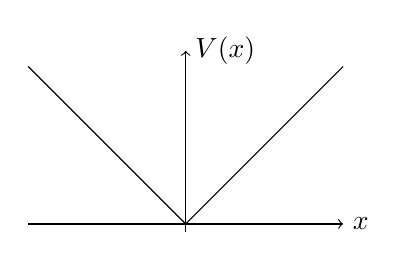
\begin{tikzpicture}
   \draw (-2,0)[->] -- (2,0) node[right] {$x$};
   \draw (0,-0.1)[->] -- (0,2.2) node[right] {$V(x)$};
   \draw (-2,2) -- (0,0) -- (2,2);
  \end{tikzpicture}
 \end{center}
\end{enumerate}

The Hamiltonian
\begin{equation*}
 H(p,x) = \frac{p^2}{2m} + k|x|
\end{equation*}
is time-independent, so the total energy $H(p,x) = E$ is conserved.  The momentum can thus be written as $p = \sqrt{2m \left(E - k|x|\right)}$.
The motion occurs between $-a$ and $+a$ with $a = \frac{E}{k}$ determined by when $p$ is zero.  To find the action we integrate over a full period of the motion,
\begin{eqnarray*}
 J = \oint p dx & = & 2 \int_{-a}^{+a} \sqrt{2m \left(E - k|x|\right)} dx \\
 & = & 2 \int_{-a}^0 \sqrt{2m \left(E + k x\right)} dx + 2 \int_0^{+a} \sqrt{2m \left(E - k x\right)} dx \\
 & = & - 2 \int_{+a}^0 \sqrt{2m \left(E - k x\right)} dx + 2 \int_0^{+a} \sqrt{2m \left(E - k x\right)} dx \\
 & = & 4 \int_0^{+a} \sqrt{2m \left(E + k x\right)} dx \\
 & = & - \frac{4\sqrt{2m}}{k} \int_0^{+a} \sqrt{\left(E - k x\right)} d(E - k x) \\
 & = & - \frac{4\sqrt{2m}}{k} \frac{2}{3} \left(E - k x\right)^\frac{3}{2}|_0^{a = \frac{E}{k}} \\
 & = & \frac{8\sqrt{2m}}{3k} E^\frac{3}{2}.
\end{eqnarray*}
We can write the energy as a function of the action.
\begin{equation*}
 H(J) = E = \left(\frac{3kJ}{8\sqrt{2m}}\right)^\frac{2}{3}.
\end{equation*}
The frequency is now
\begin{eqnarray*}
 \nu = \frac{\partial H}{\partial J} & = & \frac{2}{3} \left(\frac{3k}{8\sqrt{2m}}\right)^\frac{2}{3} J^{-\frac{1}{3}} \\
 & = & \frac{2}{3} \left(\frac{3k}{8\sqrt{2m}}\right)^\frac{2}{3} \left(\frac{8\sqrt{2m}}{3k}\right)^{-\frac{1}{3}} E^{-\frac{1}{2}} \\
 & = & \frac{2}{3} \left(\frac{3k}{8\sqrt{2m}}\right) \frac{1}{\sqrt{E}}.
\end{eqnarray*}


\end{document}
